% ------------------------------------------------------------
% LaTeX Template für die DHBW zum Schnellstart!
% Original: https://github.wdf.sap.corp/vtgermany/LaTeX-Template-DHBW
% ------------------------------------------------------------
% ---- Präambel mit Angaben zum Dokument
\documentclass[
	fontsize=12pt,           % Leitlinien sprechen von Schriftgröße 12.
	paper=A4,
	twoside=false,
	listof=totoc,            % Tabellen- und Abbildungsverzeichnis ins Inhaltsverzeichnis
	bibliography=totoc,      % Literaturverzeichnis ins Inhaltsverzeichnis aufnehmen
	titlepage,               % Titlepage-Umgebung anstatt \maketitle
	headsepline,             % horizontale Linie unter Kolumnentitel
	abstract,              % Überschrift einschalten, Abstract muss in {abstract}-Umgebung stehen
]{scrreprt}                  % Verwendung von KOMA-Report
\usepackage[utf8]{inputenc}  % UTF8 Encoding einschalten
\usepackage[ngerman]{babel}  % Neue deutsche Rechtschreibung
\usepackage[T1]{fontenc}     % Ausgabe von westeuropäischen Zeichen (auch Umlaute)
\usepackage{microtype}       % Trennung von Wörtern wird besser umgesetzt
\usepackage{lmodern}         % Nicht-gerasterte Schriftarten (bei MikTeX erforderlich)
\usepackage{graphicx}        % Einbinden von Grafiken erlauben
\usepackage{wrapfig}         % Grafiken fließend im Text
\usepackage{setspace}        % Zeilenabstand \singlespacing, \onehalfspaceing, \doublespacing
\usepackage[
	%showframe,                % Ränder anzeigen lassen
	left=2.7cm, right=2.5cm,
	top=2.5cm,  bottom=2.5cm,
	includeheadfoot
]{geometry}                      % Seitenlayout einstellen
\usepackage{scrlayer-scrpage}    % Gestaltung von Fuß- und Kopfzeilen
\usepackage{acronym}             % Abkürzungen, Abkürzungsverzeichnis
\usepackage{titletoc}            % Anpassungen am Inhaltsverzeichnis
\contentsmargin{0.75cm}          % Abstand im Inhaltsverzeichnis zw. Punkt und Seitenzahl
\usepackage[                     % Klickbare Links (enth. auch "nameref", "url" Package)
  hidelinks,                     % Blende die "URL Boxen" aus.
  breaklinks=true,               % Breche zu lange URLs am Zeilenende um
  colorlinks=true,
  urlcolor=blue,
  linkcolor=.,
  anchorcolor=.,
  citecolor=.,
  filecolor=.,
  menucolor=.,
  runcolor=.
]{hyperref}
\usepackage[hypcap=true]{caption}% Anker Anpassung für Referenzen
\urlstyle{same}                  % Aktuelle Schrift auch für URLs
% Anpassung von autoref für Gleichungen (ergänzt runde Klammern) und Algorithm.
% Anstatt "Listing" kann auch z.B. "Code-Ausschnitt" verwendet werden. Dies sollte
% jedoch synchron gehalten werden mit \lstlistingname (siehe weiter unten).
\addto\extrasngerman{%
	\def\equationautorefname~#1\null{Gleichung~(#1)\null}
	\def\lstnumberautorefname{Zeile}
	\def\lstlistingautorefname{Listing}
	\def\algorithmautorefname{Algorithmus}
	% Damit einheitlich "Abschnitt 1.2[.3]" verwendet wird und nicht "Unterabschnitt 1.2.3"
	% \def\subsectionautorefname{Abschnitt}
}

% ---- Abstand verkleinern von der Überschrift 
\renewcommand*{\chapterheadstartvskip}{\vspace*{.5\baselineskip}}

% Hierdurch werden Schusterjungen und Hurenkinder vermieden, d.h. einzelne Wörter
% auf der nächsten Seite oder in einer einzigen Zeile.
% LaTeX kann diese dennoch erzeugen, falls das Layout ansonsten nicht umsetzbar ist.
% Diese Werte sind aber gute Startwerte.
\widowpenalty10000
\clubpenalty10000

% ---- Für das Quellenverzeichnis
\usepackage[
	backend = biber,                % Verweis auf biber
	language = auto,
	style = numeric,                % Nummerierung der Quellen mit Zahlen
	sorting = none,                 % none = Sortierung nach der Erscheinung im Dokument
	sortcites = true,               % Sortiert die Quellen innerhalb eines cite-Befehls
	block = space,                  % Extra Leerzeichen zwischen Blocks
	hyperref = true,                % Links sind klickbar auch in der Quelle
	%backref = true,                % Referenz, auf den Text an die zitierte Stelle
	bibencoding = auto,
	giveninits = true,              % Vornamen werden abgekürzt
	doi=false,                      % DOI nicht anzeigen
	isbn=false,                     % ISBN nicht anzeigen
    alldates=short                  % Datum immer als DD.MM.YYYY anzeigen
]{biblatex}
\addbibresource{Inhalt/literatur.bib}
\setcounter{biburlnumpenalty}{3000}     % Umbruchgrenze für Zahlen
\setcounter{biburlucpenalty}{6000}      % Umbruchgrenze für Großbuchstaben
\setcounter{biburllcpenalty}{9000}      % Umbruchgrenze für Kleinbuchstaben
\DeclareNameAlias{default}{family-given}  % Nachname vor dem Vornamen
\AtBeginBibliography{\renewcommand{\multinamedelim}{\addslash\space
}\renewcommand{\finalnamedelim}{\multinamedelim}}  % Schrägstrich zwischen den Autorennamen
\DefineBibliographyStrings{german}{
  urlseen = {Einsichtnahme:},                      % Ändern des Titels von "besucht am"
}
\usepackage[babel,german=quotes]{csquotes}         % Deutsche Anführungszeichen + Zitate


% ---- Für Mathevorlage
\usepackage{amsmath}    % Erweiterung vom Mathe-Satz
\usepackage{amssymb}    % Lädt amsfonts und weitere Symbole
\usepackage{MnSymbol}   % Für Symbole, die in amssymb nicht enthalten sind.


% ---- Für Quellcodevorlage
\usepackage{scrhack}                    % Hack zur Verw. von listings in KOMA-Script
\usepackage{listings}                   % Darstellung von Quellcode
\usepackage{xcolor}                     % Einfache Verwendung von Farben
% -- Eigene Farben für den Quellcode
\definecolor{JavaLila}{rgb}{0.4,0.1,0.4}
\definecolor{JavaGruen}{rgb}{0.3,0.5,0.4}
\definecolor{JavaBlau}{rgb}{0.0,0.0,1.0}
\definecolor{ABAPKeywordsBlue}{HTML}{6000ff}
\definecolor{ABAPCommentGrey}{HTML}{808080}
\definecolor{ABAPStringGreen}{HTML}{4da619}
\definecolor{PyKeywordsBlue}{HTML}{0000AC}
\definecolor{PyCommentGrey}{HTML}{808080}
\definecolor{PyStringGreen}{HTML}{008080}
% -- Farben für ABAP CDS
\definecolor{CDSString}{HTML}{FF8C00}
\definecolor{CDSKeywords}{HTML}{6000ff}
\definecolor{CDSAnnotation}{HTML}{00BFFF}
\definecolor{CDSComment}{HTML}{808080}
\definecolor{CDSFunc}{HTML}{FF0000}

% -- Default Listing-Styles

\lstset{
	% Das Paket "listings" kann kein UTF-8. Deswegen werden hier 
	% die häufigsten Zeichen definiert (ä,ö,ü,...)
	literate=%
		{á}{{\'a}}1 {é}{{\'e}}1 {í}{{\'i}}1 {ó}{{\'o}}1 {ú}{{\'u}}1
		{Á}{{\'A}}1 {É}{{\'E}}1 {Í}{{\'I}}1 {Ó}{{\'O}}1 {Ú}{{\'U}}1
		{à}{{\`a}}1 {è}{{\`e}}1 {ì}{{\`i}}1 {ò}{{\`o}}1 {ù}{{\`u}}1
		{À}{{\`A}}1 {È}{{\'E}}1 {Ì}{{\`I}}1 {Ò}{{\`O}}1 {Ù}{{\`U}}1
		{ä}{{\"a}}1 {ë}{{\"e}}1 {ï}{{\"i}}1 {ö}{{\"o}}1 {ü}{{\"u}}1
		{Ä}{{\"A}}1 {Ë}{{\"E}}1 {Ï}{{\"I}}1 {Ö}{{\"O}}1 {Ü}{{\"U}}1
		{â}{{\^a}}1 {ê}{{\^e}}1 {î}{{\^i}}1 {ô}{{\^o}}1 {û}{{\^u}}1
		{Â}{{\^A}}1 {Ê}{{\^E}}1 {Î}{{\^I}}1 {Ô}{{\^O}}1 {Û}{{\^U}}1
		{œ}{{\oe}}1 {Œ}{{\OE}}1 {æ}{{\ae}}1 {Æ}{{\AE}}1 {ß}{{\ss}}1
		{ű}{{\H{u}}}1 {Ű}{{\H{U}}}1 {ő}{{\H{o}}}1 {Ő}{{\H{O}}}1
		{ç}{{\c c}}1 {Ç}{{\c C}}1 {ø}{{\o}}1 {å}{{\r a}}1 {Å}{{\r A}}1
		{€}{{\euro}}1 {£}{{\pounds}}1 {«}{{\guillemotleft}}1
		{»}{{\guillemotright}}1 {ñ}{{\~n}}1 {Ñ}{{\~N}}1 {¿}{{?`}}1,
	breaklines=true,        % Breche lange Zeilen um 
	breakatwhitespace=true, % Wenn möglich, bei Leerzeichen umbrechen
	% Symbol für Zeilenumbruch einfügen
	prebreak=\raisebox{0ex}[0ex][0ex]{\ensuremath{\rhookswarrow}},
	postbreak=\raisebox{0ex}[0ex][0ex]{\ensuremath{\rcurvearrowse\space}},
	tabsize=4,                                 % Setze die Breite eines Tabs
	basicstyle=\ttfamily\small,                % Grundsätzlicher Schriftstyle
	columns=fixed,                             % Besseres Schriftbild
	numbers=left,                              % Nummerierung der Zeilen
	%frame=single,                             % Umrandung des Codes
	showstringspaces=false,                    % Keine Leerzeichen hervorheben
	keywordstyle=\color{blue},
	ndkeywordstyle=\bfseries\color{darkgray},
	identifierstyle=\color{black},
	commentstyle=\itshape\color{JavaGruen},   % Kommentare in eigener Farbe
	stringstyle=\color{JavaBlau},             % Strings in eigener Farbe,
	captionpos=b,                             % Bild*unter*schrift
	xleftmargin=5.0ex
}

% ---- Eigener JAVA-Style für den Quellcode
\renewcommand{\ttdefault}{pcr}               % Schriftart, welche auch fett beinhaltet
\lstdefinestyle{EigenerJavaStyle}{
	language=Java,                             % Syntax Highlighting für Java
	%frame=single,                             % Umrandung des Codes
	keywordstyle=\bfseries\color{JavaLila},    % Keywords in eigener Farbe und fett
	commentstyle=\itshape\color{JavaGruen},    % Kommentare in eigener Farbe und italic
	stringstyle=\color{JavaBlau}               % Strings in eigener Farbe
}

% ---- Eigener ABAP-Style für den Quellcode
\renewcommand{\ttdefault}{pcr}
\lstdefinestyle{EigenerABAPStyle}{
	language=[R/3 6.10]ABAP,
	morestring=[b]\|,                          % Für Pipe-Strings
	morestring=[b]\`,                          % für Backtick-Strings
	keywordstyle=\bfseries\color{ABAPKeywordsBlue},
	commentstyle=\itshape\color{ABAPCommentGrey},
	stringstyle=\color{ABAPStringGreen},
	tabsize=2,
	morekeywords={
		types,
		@data,
		as,
		lower,
		start,
		selection,
		order,
		by,
		inner,
		join,
		key,
		end,
		cast
	}
}

% ---- Eigener Python-Style für den Quellcode
\renewcommand{\ttdefault}{pcr}
\lstdefinestyle{EigenerPythonStyle}{
	language=Python,
	columns=flexible,
	keywordstyle=\bfseries\color{PyKeywordsBlue},
	commentstyle=\itshape\color{PyCommentGrey},
	stringstyle=\color{PyStringGreen}
}

%----- ABAP-CDS-View language
\lstdefinelanguage{ABAPCDS}{
	sensitive=false,
	%Keywords
	morekeywords={define,
		view,
		as,
		select,
		from,
		inner,
		join,
		on,
		key,
		case,
		when,
		then,
		else,
		end,
		true,
		false,
		cast,
		where,
		and,
		distinct,
		group,
		by,
		having,
		min,
		sum,
		max,
		count,
		avg
	},
	%Methoden
	morekeywords=[2]{
		div,
		currency\_conversion,
		dats\_days\_between,
		concat\_with\_space,
		dats\_add_days,
		dats\_is\_valid,
		dats\_add\_months,
		unit\_conversion,
		division,
		mod,
		abs,
		floor,
		ceil,
		round,
		concat,
		replace,
		substring,
		left,
		right,
		length
	},
	morecomment=[s][\color{CDSAnnotation}]{@}{:},
	morecomment=[l][\itshape\color{CDSComment}]{//},
	morecomment=[s][\itshape\color{CDSComment}]{/*}{*/},
	morestring=[b][\color{CDSString}]',
	keywordstyle=\bfseries\color{CDSKeywords},
	keywordstyle=[2]\color{CDSFunc}
}

  % Weitere Details sind ausgelagert

\usepackage{algorithm}                  % Für Algorithmen-Umgebung (ähnlich wie lstlistings Umgebung)
\usepackage{algpseudocode}              % Für Pseudocode. Füge "[noend]" hinzu, wenn du kein "endif",
                                        % etc. haben willst.

\makeatletter                           % Sorgt dafür, dass man @ in Namen verwenden kann.
                                        % Ansonsten gibt es in der nächsten Zeile einen Compilefehler.
\renewcommand{\ALG@name}{Algorithmus}   % Umbenennen von "Algorithm" im Header der Listings.
\makeatother                            % Zeichen wieder zurücksetzen
\renewcommand{\lstlistingname}{Listing} % Erlaubt das Umbenennen von "Listing" in anderen Titel.

% ---- Tabellen
\usepackage{booktabs}  % Für schönere Tabellen. Enthält neue Befehle wie \midrule
\usepackage{multirow}  % Mehrzeilige Tabellen
\usepackage{siunitx}   % Für SI Einheiten und das Ausrichten Nachkommastellen
\sisetup{locale=DE, range-phrase={~bis~}, output-decimal-marker={,}} % Damit ein Komma und kein Punkt verwendet wird.
\usepackage{xfrac} % Für siunitx Option "fraction-function=\sfrac"

% ---- Für Definitionsboxen in der Einleitung
\usepackage{amsthm}                     % Liefert die Grundlagen für Theoreme
\usepackage[framemethod=tikz]{mdframed} % Boxen für die Umrandung
% ---- Definition für Highlight Boxen

% ---- Grundsätzliche Definition zum Style
\newtheoremstyle{defi}
  {\topsep}         % Abstand oben
  {\topsep}         % Abstand unten
  {\normalfont}     % Schrift des Bodys
  {0pt}             % Einschub der ersten Zeile
  {\bfseries}       % Darstellung von der Schrift in der Überschrift
  {:}               % Trennzeichen zwischen Überschrift und Body
  {.5em}            % Abstand nach dem Trennzeichen zum Body Text
  {\thmname{#3}}    % Name in eckigen Klammern
\theoremstyle{defi}

% ------ Definition zum Strich vor eines Texts
\newmdtheoremenv[
  hidealllines = true,       % Rahmen komplett ausblenden
  leftline = true,           % Linie links einschalten
  innertopmargin = 0pt,      % Abstand oben
  innerbottommargin = 4pt,   % Abstand unten
  innerrightmargin = 0pt,    % Abstand rechts
  linewidth = 3pt,           % Linienbreite
  linecolor = gray!40,       % Linienfarbe
]{defStrich}{Definition}     % Name der des formats "defStrich"

% ------ Definition zum Eck-Kasten um einen Text
\newmdtheoremenv[
  hidealllines = true,
  innertopmargin = 6pt,
  linecolor = gray!40,
  singleextra={              % Eck-Markierungen für die Definition
    \draw[line width=3pt,gray!50,line cap=rect] (O|-P) -- +(1cm,0pt);
    \draw[line width=3pt,gray!50,line cap=rect] (O|-P) -- +(0pt,-1cm);
    \draw[line width=3pt,gray!50,line cap=rect] (O-|P) -- +(-1cm,0pt);
    \draw[line width=3pt,gray!50,line cap=rect] (O-|P) -- +(0pt,1cm);
  }
]{defEckKasten}{Definition}  % Name der des formats "defEckKasten"  % Weitere Details sind ausgelagert

% ---- Für Todo Notes
\usepackage{todonotes}
\setlength {\marginparwidth }{2cm}      % Abstand für Todo Notizen

\usepackage[htt]{hyphenat}
\usepackage{dirtree,array}
\renewcommand\DTstyle{\fontsize{9}{11}\rmfamily}

\usepackage{float}

% ---- Elektronische Version oder Gedruckte Version?
% ---- Unterschied: Die elektronische Version enthält keinen Platzhalter für die Unterschrift
\usepackage{ifthen}
\newboolean{e-Abgabe}
\setboolean{e-Abgabe}{false}    % false=gedruckte Fassung

% ---- Persönlichen Daten:
\newcommand{\titelheader}{Programmentwurf}
\newcommand{\bearbeitende}{Yannik Schiebelhut}

% ---- Metainformation für das PDF Dokument
\hypersetup{
	pdftitle    = {Software Engineering II (TINF19B1)},
	pdfsubject  = {Programmentwurf},
	pdfauthor   = {\bearbeitende},
	%pdfkeywords = {Keywords angeben},
	pdfcreator  = {LaTeX},
	%pdfproducer = {in der Regel pdfTeX}
}

% ---- Definition der Kopf- und Fußzeilen
\clearpairofpagestyles                          % Löschen von LaTeX Standard
\automark[section]{chapter}                     % Füllen von section und chapter
\renewcommand*{\chaptermarkformat}{}            % Entfernt die Kapitelnummer
\renewcommand*{\sectionmarkformat}{}            % Entfernt die Sectionnummer
% Angaben [für "plain"]{für "scrheadings"}
\ihead[]{\titelheader}                          % Kopfzeile links
\chead[]{}                                      % Kopfzeile mitte
\ohead[]{\rightmark}                            % Kopfzeile rechts
\ifoot[]{}                                      % Fußzeile links
\cfoot*{\sffamily\pagemark}                     % Fußzeile mitte
\ofoot[]{}                                      % Fußzeile rechts
\KOMAoptions{
   headsepline = 0.2pt,                         % Liniendicke Kopfzeile
   footsepline = false                          % Liniendicke Fußzeile
}


% ---- Hilfreiches
\newcommand{\zB}{z.\,B. }   % "z.B." mit kleinem Leeraum dazwischen (ohne wäre nicht korrekt)
\newcommand{\dash}{d.\,h. }

\newcommand{\code}[1]{\texttt{#1}} % Ist einfacher zu schreiben als ständig \texttt und erlaubt
                                   % Änderungen im Nachhinein, wenn man z.B. Inline-Code anders stylen möchte.

% ---- Silbentrennung (falls LaTeX defaults falsch / nicht gewünscht sind)
\hyphenation{HANA}         % anstatt HA-NA
\hyphenation{Graph-Script} % anstatt GraphS-cript

% ---- Beginn des Dokuments
\begin{document}
\setlength{\parindent}{0pt}              % Keine Paragraphen Einrückung.
                                         % Dafür haben wir den Abstand zwischen den Paragraphen.
\setcounter{secnumdepth}{2}              % Nummerierungstiefe fürs Inhaltsverzeichnis
\setcounter{tocdepth}{1}                 % Tiefe des Inhaltsverzeichnisses. Ggf. so anpassen,
                                         % dass das Verzeichnis auf eine Seite passt.
\sffamily                                % Serifenlose Schrift verwenden.

% ---- Vorspann
% ------ Titelseite
\singlespacing
\thispagestyle{empty}
\begin{titlepage}
\enlargethispage{4cm}

\begin{figure}           % Logo vom Ausbildungsbetrieb und der DHBW
	% \vspace*{-5mm} % Sollte dein Titel zu lang werden, kannst du mit diesem "Hack" 
	%                  den Inhalt der Seite nach oben schieben.
	\begin{minipage}{0.49\textwidth}
		\flushleft
		%\includegraphics[width=0.9\textwidth]{Bilder/Logos/Logo.pdf} 
	\end{minipage}
	\hfill
	\begin{minipage}{0.49\textwidth}
		\flushright
		
\includegraphics[height=2.5cm]{Bilder/Logos/Logo_DHBW.pdf} 
	\end{minipage}
\end{figure} 
\vspace*{0.1cm}

\begin{center}
	\huge{\textbf{Software-Engineering II}}\\[1.5cm]
	\Large{\textbf{Programmentwurf}}\\
	\Large{\textbf{TINF20B1}}\\
	\Large{\textbf{5.$+$6. Semester (2022/2023)}}\\[1cm]
	\Large{\textbf{Thema:}}\\
	\Large{\textbf{Kostenrechner für Fahrgemeinschaften}}\\[2cm]
\end{center}

\begin{center}
	\normalsize{Dozent:}\\
	\large{Daniel Lindner}
\end{center}

\begin{center}
	\normalsize{Bearbeitender:}\\
	\Large{\bearbeitende}
\end{center}
\end{titlepage}
  % Titelseite
\newcounter{savepage}
\pagenumbering{Roman}                    % Römische Seitenzahlen
\onehalfspacing

% ------ Inhaltsverzeichnis
\singlespacing
\tableofcontents

% ------ Verzeichnisse
\renewcommand*{\chapterpagestyle}{plain}
\pagestyle{plain}
\chapter*{Abkürzungsverzeichnis}
\addcontentsline{toc}{chapter}{Abkürzungsverzeichnis} % Hinzufügen zum Inhaltsverzeichnis 

\begin{acronym}[WYSISWG] % längstes Kürzel wird verw. für den Abstand zw. Kürzel u. Text

	% Alphabetisch selbst sortieren - nicht verwendete Kürzel rausnehmen!
	% \acro{API}{Application Programming Interface}
    % \acro{CLI}{Command Line Interface}
    % \acro{IDE}{Integrated Development Environment}
    % \acro{JPA}{Java Persistence API}

\end{acronym}

\listoffigures                          % Erzeugen des Abbildungsverzeichnisses 
\setcounter{savepage}{\value{page}}


% ---- Inhalt der Arbeit
\cleardoublepage
\pagenumbering{arabic}                  % Arabische Seitenzahlen für den Hauptteil
\setlength{\parskip}{0.5\baselineskip}  % Abstand zwischen Absätzen
\rmfamily
\renewcommand*{\chapterpagestyle}{scrheadings}
\pagestyle{scrheadings}
\onehalfspacing
\chapter{Beschreibung des Programms}
Im Rahmen eines dualen Studiums an der DHBW bietet es sich an, für die Praxisphasen mit anderen Studenten Fahrgemeinschaften zum Betrieb zu bilden.
Diese Fahrgemeinschaften haben zwar einen festen Rahmen an Mitgliedern, jedoch haben diese alle verschiedene und wechselnde Termine, wodurch sich der Anwendungsfall für ein Programm ergeben hat, welches den Fahrer einer Fahrgemeinschaft dabei unterstützt, mit wenig Aufwand eine für alle Beteiligten faire Abrechnung zu erstellen.

\section{Funktionalität}
\label{sec:funktionalität}
Das Programm richtet sich an den Besitzer eines Autos, weiterhin als Fahrer bezeichnet.
Der Fahrer kann mehrere \enquote{Fahrgemeinschaften}, also Gruppen von Personen, definieren.
Dabei kann eine Person in mehreren Fahrgemeinschaften sein und eine Fahrgemeinschaft hat in der Regel mehrere Mitfahrer.

Innerhalb einer Fahrgemeinschaft werden Fahrperioden angelegt.
Eine Fahrperiode bezeichnet dabei die Menge aller Fahrten zwischen zwei Tankstopps.
Innerhalb einer Fahrperiode haben alle Fahrten dieselbe Strecke, denselben Spritverbrauch und denselben Spritpreis.
Des Weiteren kann ein Fixbetrag definiert werden, um etwa Verschleißkosten des Fahrzeugs auf die Mitfahrer umzulegen.
In einer Fahrperiode wiederum kann eine beliebige Menge an Fahrten angelegt werden.
Für jede dieser Fahrten wird ausgewählt, welche Mitglieder der Fahrgemeinschaft im Fahrzeug saßen.
Wenn wieder getankt wird, wird die Fahrperiode im System abgeschlossen.
Dabei wird der Anteil an den entstandenen Fahrkosten für jeden Mitfahrer innerhalb der Fahrperiode ermittelt.
Für diesen Anteil wird ein PayPal-Link generiert und der jeweiligen Person über Telegram zugesandt, um auch den Bezahlvorgang angenehm zu gestalten.

Eine Person wiederum hat einen Namen, eine Adresse und eine Telegram-Chat-ID, über die diese Person zu kontaktieren ist.

\section{Technologien}
Umgesetzt ist das Programm in Java, wobei Maven als Build-System verwendet wird.
Die Datenhaltung erfolgt lokal im JSON-Format mittels der externen GSON-Bibliothek.
Das Programm verfügt über eine grafische Nutzeroberfläche, welche mit Java Swing erstellt ist.
Weiterhin wird auf die Telegram API zugegriffen.
Hierfür ist allerdings im Rahmen einer einfachen Proof of Concept Implementierung keine externe Bibliothek vonnöten.

Der Quellcode wird in einem Git-Repository verwaltet, welches auf GitHub unter \url{https://github.com/yschiebelhut/carpool-java} zu finden ist.
\chapter{Domain Driven Design}
\chapter{Clean Architecture}
In diesem Kapitel wird die Software so in verschiedene Teilmodule restrukturiert, dass sie den Grundsätzen der in der Vorlesung vermittelten Clean Architecture genügt.

\section{Unterteilung in Schichten}
\subsection{Schicht 4: Abstraction Code}
\emph{Abstraction Code} stellt domänenübergreifendes Wissen dar (wie etwa mathematische Konzepte, grundlegende Algorithmen oder Datenstrukturen).
Im Kontext der vorliegenden Software wird diese Schicht nicht benötigt.
Mathematische Konzepte, die zur Berechnung der Fahrtkosten notwendig sind, sowie alle in der Software verwendeten Datenstrukturen, finden sich bereits in den Java-Bibliotheken.

\subsection{Schicht 3: Domain}
In dieser Schicht wird der zentrale Domain-Code untergebracht.
In diesem Falle sind dies die in \autoref{fig:domainmodel} gezeigten und im vorherigen Kapitel beschriebenen Entitäten und Value Objects (implementiert im Modul \code{3-carpool-java-domain}).
Sie gehören zur elementaren Business Logik der Domaine und sollten sich möglichst selten, in der Regel eigentlich nie ändern.
Lediglich das in der Abbildung dargestellte \emph{Integration} Package wird in die Schicht 0 verschoben.
Zwar gehört gemäß Beschreibung des Domainen-Experten das Senden von PayPal-Links via Telegram als elementarer Bestandteil zum Programm, jedoch sollte die konkrete Implementierung der Interaktion mit diesen Diensten nicht als Teil des Domainen-Codes erfolgen, da sich diese logisch abgrenzt und Änderungen im Laufe der Zeit sehr wahrscheinlich sind.

\subsection{Schicht 2: Application}
Die Application-Schicht ist gemäß der Vorlesung für Aggregat-übergreifendes Verhalten verantwortlich.
In Falle der vorliegenden Software liegt dieser Anwendungsfall beim Versenden der PayPal-Links über Telegram vor.
Hierbei werden die Rechnungsdaten einer Fahrperiode ausgelesen.
Diese enthalten jedoch nur ein Mapping einer UUID zu einem Geldbetrag.
Zum Versenden der Nachrichten müssen diese UUIDs noch zu Personen aufgelöst werden, aus welchen anschließend die Telegram-Chat-ID extrahiert werden kann.
Umgesetzt ist diese Schicht im Modul \code{2-carpool-java-application}.

\subsection{Schicht 1: Adapters}
Die Adapters-Schicht soll in der Clean Architecture dazu dienen, Aufrufe und Daten der Plugin-Schicht an die innere Schicht zu vermitteln.
Hier finden zum Beispiel Aufgaben wie Formatkonvertierungen und das Erstellen von Render-Modellen statt.
Da jedoch in der Plugin-Schicht dieser Anwendung keine komplexe Umsetzungslogik erfolgt und ein Erstellen dieser Schicht keinen unmittelbaren Wert besitzt (wie auf Folie 49 der Clean Architecture beschrieben), wird auf das Erstellen dieser Schicht verzichtet.
Es ist allerdings darauf hinzuweisen, dass ein Erstellen dieser Schicht theoretisch empfehlenswert wäre, vor allem in der Hinsicht, dass die aktuell mit Java-Swing erstellte Benutzeroberfläche nicht gerade schön ist und gegebenenfalls zukünftig durch eine neuere und bessere Oberfläche ersetzt werden könnte.
Eine solche Oberfläche kann ohne die Adapters-Schicht nicht auf visuelle Verarbeitungsroutinen der aktuellen GUI zugreifen und müssten neu angefertigt werden, was wiederum mit einem Mehraufwand verknüpft wäre.

\subsection{Schicht 0: Plugins}
Die Plugin-Schicht stellt die äußerste Schicht der Anwendung dar.
Code in dieser Schicht ist am kurzlebigsten.
Hier werden für die aktuelle Anwendung 4 Module erstellt: \code{0-carpool-java-plugins-main}, \code{0-carpool-java-plugins-ui}, \code{0-carpool-java-plugins-json} und \code{0-carpool-java-plugins-integration}.

\subsubsection{Main-Plugin}
Dieses Plugin enthält die Main-Methode und somit den Einstiegspunkt in die Applikation.
Hier ist keinerlei Anwendungslogik enthalten, sondern es erfolgt lediglich eine Koordinierung der anderen Plugins.
Die Main-Methode delegiert die Datenverwaltung an das JSON-Plugin und initialisiert die vom GUI-Plugin implementierte Benutzeroberfläche.
Weiterhin wird ein Runtime-Hook definiert, der dafür sorgt, dass beim Beenden der Anwendung die aktuellen Daten gespeichert werden.
Das Speichern wird somit vom Lebenszyklus der GUI entkoppelt.

\subsubsection{GUI-Plugin}
Hier findet die Implementierung der GUI statt.
Da die Benutzeroberfläche Pure Fabrication darstellt und häufige Änderungen und Wechsel zu erwarten sind, wird diese in der Plugin-Schicht implementiert.

\subsubsection{JSON-Plugin}
Die Software setzt aktuell auf eine JSON-basierte Datenhaltung.
Zu diesem Zwecke wird die externe GSON-Library verwendet.
Weil eine externe Library eingebunden wird und die Form der Datenhaltung sehr einfach veränderlich sein sollte, wird die Datenhaltung als Plugin implementiert.
Dabei werden zwei Repository-Klassen erstellt, die die in der Domain-Schicht definierten Interfaces implementieren.
Für das Speichern gewisser Datentypen wie beispielsweise \code{LocalDate} aus der Java-Standardlibrary werden von GSON Typadapter benötigt.
Theoretisch wären diese der Adapters-Schicht zuzuordnen.
Allerdings sind die enthaltenen Mappings speziell auf die Verwendung mit GSON zuzuschneiden.
Weiterhin müssen die Adapter Interfaces implementieren, die von der Library definiert werden.
Aus diesen Gründen ist es nicht sinnvoll, die Typadapter in die Adapter-Schicht auszulagern.

\subsubsection{Integration-Plugin}
In diesem Plugin werden die PayPal-Link-Generierung sowie die Interaktion mit Telegram implementiert.
Beides bezieht sich auf Schnittstellen von externen Systemen, von denen perse schon ein häufiger Wandel zu erwarten ist, weshalb diese Klassen auf jeden Fall in der Pluin-Schicht zu implementieren sind.

\section{Dependency Inversion}
Als zentrale Regel der Clean Architecture (Dependency Rule) sollten Abhängigkeiten nur von außen nach innen zeigen.
Bis auf eine Ausnahme ist diese Regel nach der Umstrukturierung bereits erfüllt.

Die Klasse \code{FahrperiodenAbschliessService} aus \code{2-carpool-java-application} hat jedoch eine Abhängigkeit auf die Klassen \code{Telegram} und \code{PayPalLinkBuilder} aus der Schicht \code{0-carpool-java-plugins-integration}.
Um diese Abhängigkeit zu beseitigen wird eine Dependency Inversion durchgeführt.

Hierfür werden zunächst in \code{2-carpool-java-application} zwei Interfaces (\code{TelegramClient} und \code{IPayPalLinkBuilder}) definiert.
Diese Interfaces deklarieren die Methoden der beiden Klassen aus Schicht 0.
Anschließend wird eine Abhängigkeit definiert, die vom Plugin zur Applikationsschicht zeigt.
Anschließend wird die Implementierung der beiden betroffenen Klassen in Schicht 0 so verändert, dass das jeweils korrespondierte Interface implementiert wird.
Weiterhin muss der \code{FahrperiodenAbschliessService} so modifiziert werden, dass die Abhängigkeiten per Dependency Injection übergeben werden.
Der Konstruktoraufruf ist entsprechend anzupassen.

(Es ist darauf hinzuweisen, dass dadurch im vorliegenden Fall eine neue Abhängigkeit des GUI-Plugins auf das Integrations-Plugin entsteht.
Theoretisch wäre es optimal, auch diese zu vermeiden.
Da diese neue Abhängigkeit jedoch die Dependency Rule nicht verletzt und der Aufwand zur Vermeidung unverhältnismäßig hoch wäre, wird auf eine Umsetzung verzichtet.)
\chapter{Entwurfsmuster}
Entwurfsmuster dienen in der Softwareentwicklung als Lösungsansätze für wiederkehrende Probleme.
Es handelt sich dabei nicht um fertigen Code, sondern vielmehr um konzeptionelle Bausteine, die zum Beispiel die Kommunikation unter Entwicklern unterstützen können.
Auch in diesem Programmentwurf finden sich Entwurfsmuster wieder.
Im Folgenden wird eines dieser Entwurfsmuster genauer erläutert.

\section{Beobachter}
Der Beobachter gehört zur Kategorie der Verhaltensmuster.
Kern des Konzeptes ist es, Änderungen an einem Ausgangsobjekt einer Anzahl anderer Objekte mitzuteilen.
Im Gegensatz zum Polling (ein Objekt fragt periodisch ab, ob sich der Zustand eines anderen geändert hat) findet hier Kommunikation nur im Änderungsfall statt.

Kernelement des Entwurfsmusters sind Subjekte, die von den Beobachtern observiert werden.
Ein Subjekt hat dabei die Möglichkeit, Beobachter an- und abzumelden, sowie diese zu benachrichtigen, wenn eine Veränderung vorliegt.
Bei dieser Benachrichtigung wird über alle registrierten Beobachter iteriert und deren Methode zur Aktualisierung aufgerufen.
Je nach Implementierung des Entwurfsmusters kann hier auch eine Payload mitgegeben werden.
Eine Darstellung des allgemeinen Schemas ist in \autoref{fig:beobachter-muster} zu sehen.

\begin{figure}
    \centering
    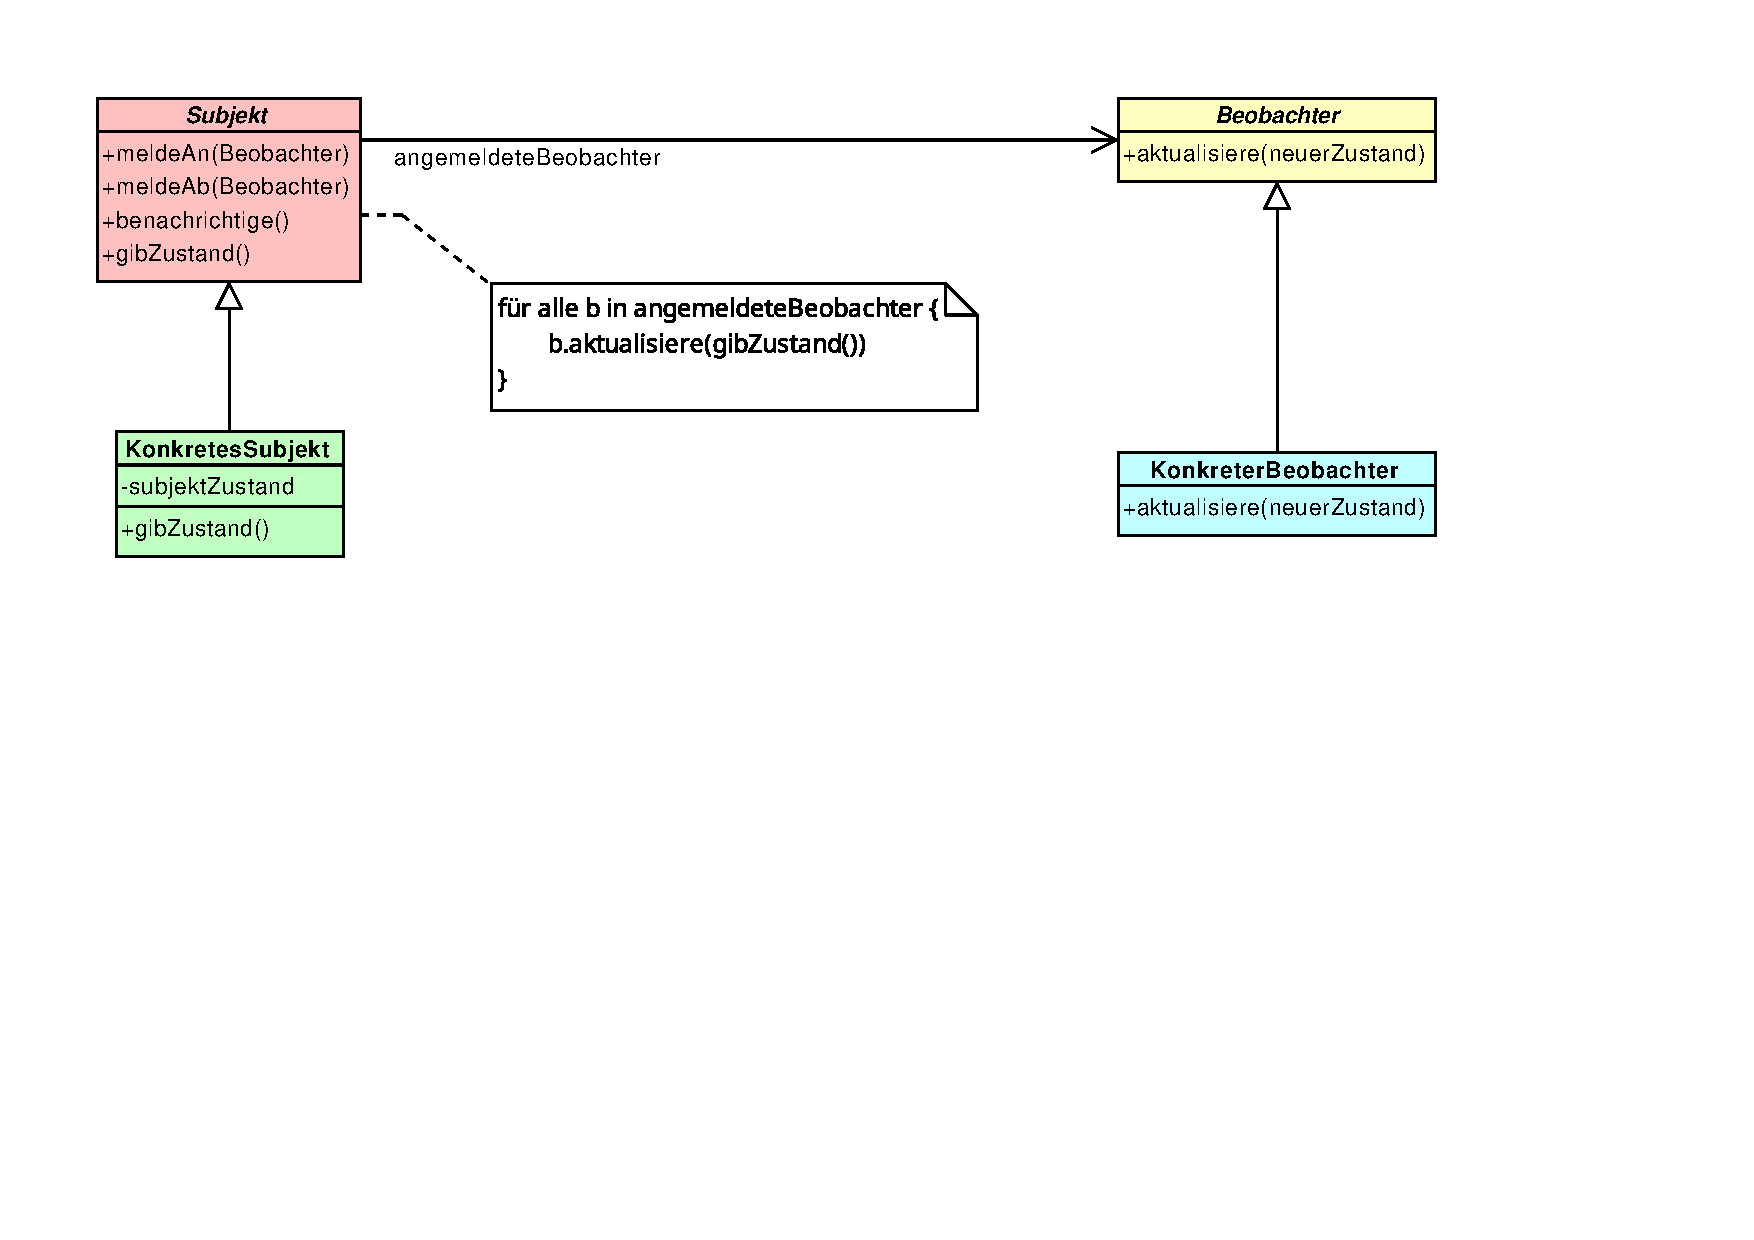
\includegraphics[width=\textwidth, trim = 0cm 10cm 3.5cm 0cm]{../VPP/Beobachter-Muster.pdf}
    \caption{Abstraktes UML-Diagramm des Beobachter-Entwurfsmusters}
    \label{fig:beobachter-muster}
\end{figure}

\subsection{Umsetzung im Programmentwurf}
In der grafischen Benutzeroberfläche des Fahrtkostenrechners spielen Knöpfe (JButtons) eine wichtige Rolle.
Knöpfe werden dabei ohne eigene Funktionalität instanziiert.
Stattdessen können für einen Knopf sogenannte \emph{ActionListener} registriert werden.
Dieser Vorgang (in \autoref{fig:beobachter-umsetzung} dargestellt) entspricht dem Beobachter-Entwurfsmuster.
Es wurde farblich hervorgehoben, welche Klassen der Umsetzung welcher Rolle des allgemeinen Schemas entsprechen.
\code{AbstractButton} entspricht dem abstrakten \code{Subjekt}, \code{ActionListener} dem abstrakten \code{Beobachter}, wobei hier für den abstrakten Beobachter ein Interface herangezogen wird anstelle einer Klasse.
Dieses Interface wird dann von der Klasse \code{FahrperiodenAbschliessService} implementiert.
\code{JButton} stellt die Implementierung des konkreten Subjekts (\code{KonkretesSubjekt}) dar.

\paragraph{Anmerkung}
\autoref{fig:beobachter-umsetzung} ist eine vereinfachte Darstellung der Implementierung des Java-Standards.
Insbesondere bei der Darstellung der \code{listenerList} wurde die Komplexität auf das Wesentliche heruntergebrochen, da die eigentliche Detailtiefe der Implementierung für die reine Demonstration des Entwurfsmusters hinderlich ist.

Die Verwendung des Entwurfsmusters ist \href{https://github.com/yschiebelhut/carpool-java/blob/fcc3bbaff5e8908a5f768b7fd3e79f1d2285acb6/0-carpool-java-plugin-ui/src/main/java/gui/FahrperiodeGUI.java#L103}{hier (Instanziierung des JButtons / Registrierung des ActionListeners)} und \href{https://github.com/yschiebelhut/carpool-java/blob/fcc3bbaff5e8908a5f768b7fd3e79f1d2285acb6/2-carpool-java-application/src/main/java/services/FahrperiodenAbschliessService.java}{hier (Implementierung des ActionListeners)} zu finden.
Die Implementierung der Subjekte ist Teil des Java-Standards.

\begin{figure}
    \centering
    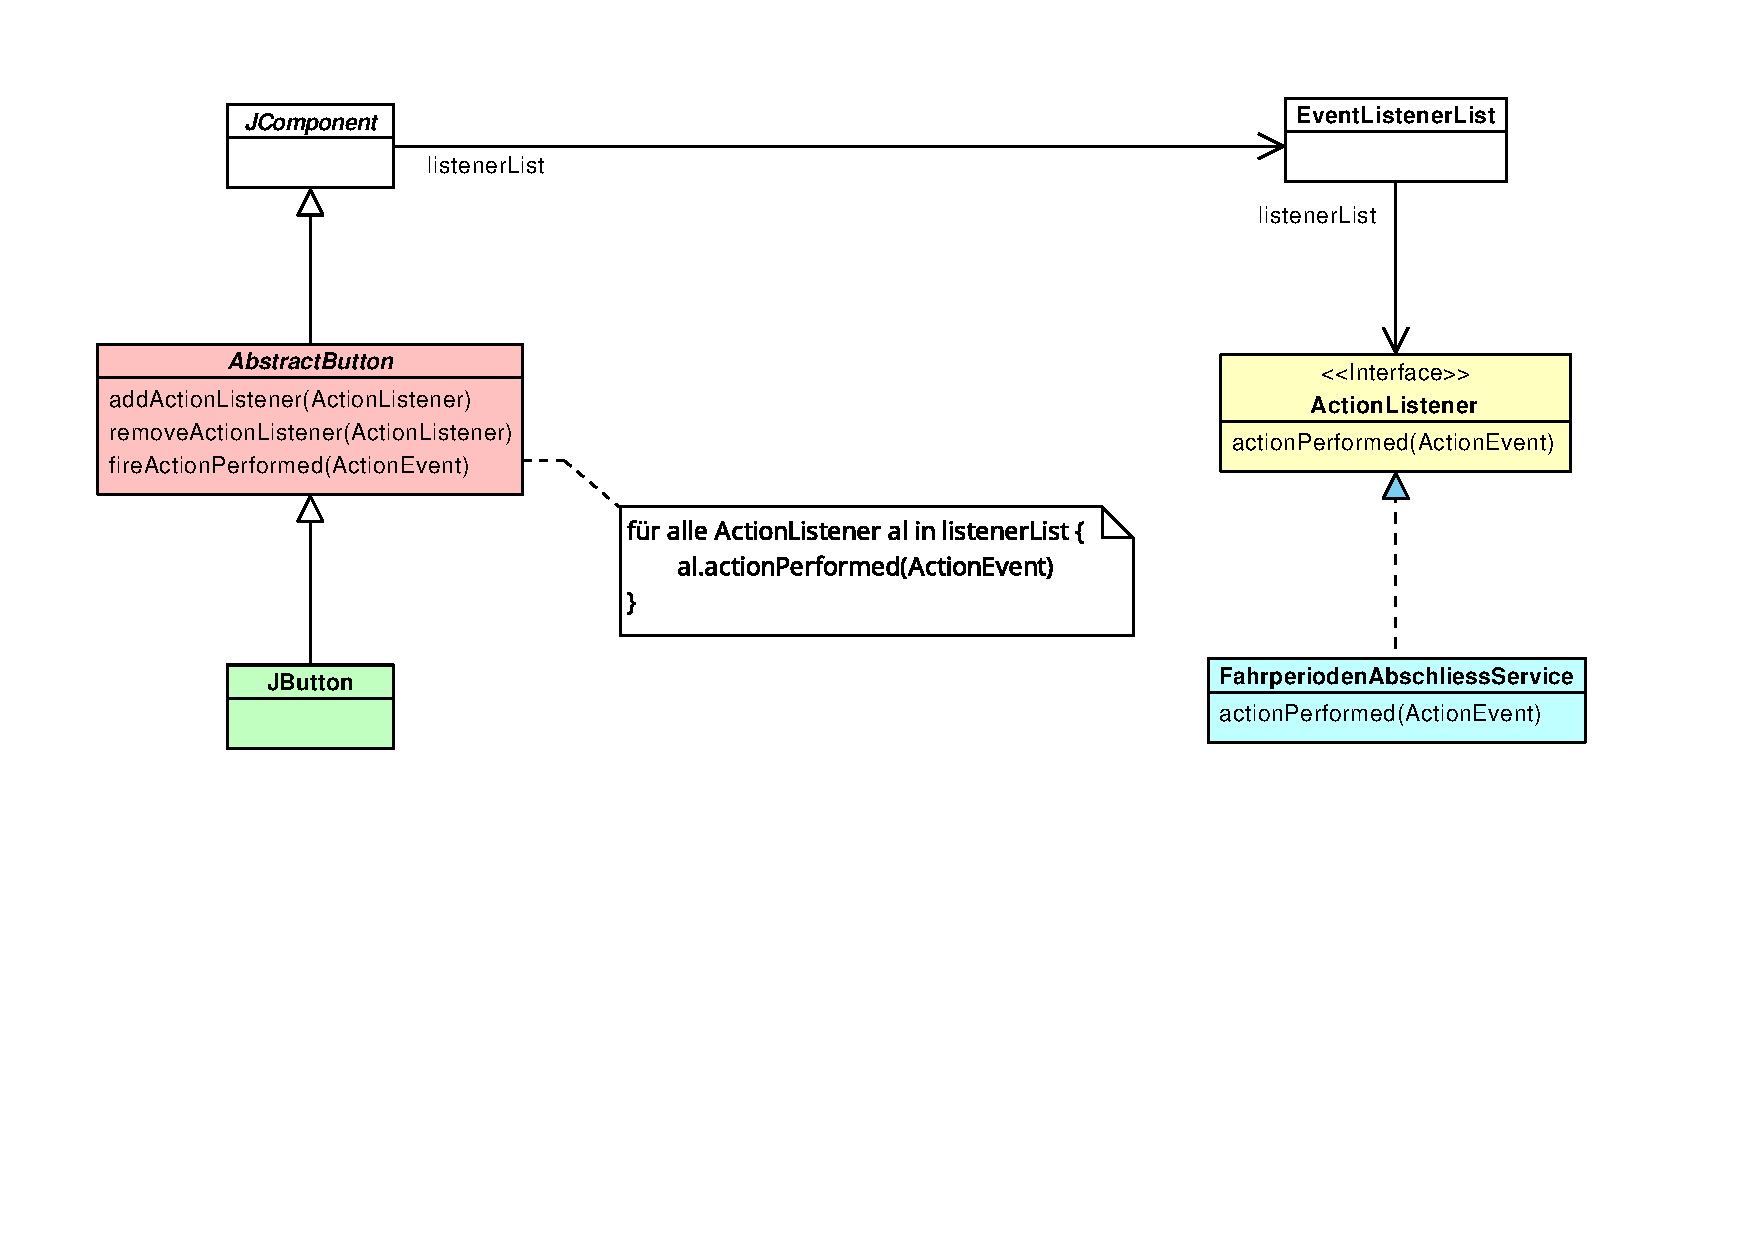
\includegraphics[width=\textwidth, trim = 0cm 7cm 0cm 0cm]{../VPP/Beobachter-Umsetzung.pdf}
    \caption{Konkrete Anwendung des Beobachter-Entwurfsmusters}
    \label{fig:beobachter-umsetzung}
\end{figure}
\chapter{Unit-Tests}
Zur zukünftigen Qualitätssicherung und frühzeitigen Erkennung von Fehlern wurden im Rahmen des Programmentwurfs an einigen sinnvollen Stellung exemplarische Unit-Tests implementiert.
Zum Einsatz kamen hier JUnit 5, AssertJ sowie EasyMock.
\autoref{fig:uebersicht} stellt eine Übersicht über die erstellten Unit-Tests dar.

\begin{figure}[H]
    \centering
    \includegraphics[width=0.5\textwidth]{Bilder/Übersicht-Unit-Tests.png}
    \caption{Übersicht über die erstellen Unit-Tests}
    \label{fig:uebersicht}
\end{figure}

\section{ATRIP-Regeln}
Die ATRIP-Regeln bieten Richtlinien, die bei der Erstellung von guten und nachhaltigen Unit-Tests unterstützen sollen.

\subsection{Automatic}
\label{sec:automatic}
Die Automatic-Regel besagt, dass Tests eigenständig ausführbar sein sollten.
Dies inkludiert eine selbstständige Überprüfung der Ergebnisse sowie auch eine Unabhängigkeit von Nutzerinteraktion, wie etwa Eingabedialogen.
Grundsätzlich wurden alle Tests so konzipiert, dass sie gemäß den genannten Kriterien automatisch ablaufen.

Allerdings ist anzumerken, dass zwar die Durchführung aller Tests automatisiert ist, es jedoch bei den \href{https://github.com/yschiebelhut/carpool-java/blob/d0315b99dcd93e582ef60fddb185b7962bcb0076/0-carpool-java-integration/src/test/java/paypal/PayPalLinkBuilderTest.java}{Tests des PayPalLinkBuilders} zu einem Problem kommt.
Für den Einsatz der Klasse PayPalLinkBuilder wird vorausgesetzt, dass die Umgebungsvariable \code{PAYPAL\_USERNAME} (auf den Wert \code{testuser}) gesetzt ist.
In anderen Programmiersprachen (etwa Node.js) stellt es (auch Plattform-übergreifend) kein Problem dar, aus einem laufenden Prozess Umgebungsvariablen zu setzen.
Somit könnte der Test diese Variable bei der Ausführung selbstständig auf den erforderlichen Wert setzen.
Java hingegen betrachtet die Umgebungsvariablen, mit denen die JVM aufgerufen wurde, als immutable, weshalb sie zur Laufzeit nicht verändert werden können.
Deshalb muss der Test mit einer vorab erstellten Run-Configuration ausgeführt werden, die sicherstellt, dass die Umgebungsvariable auf den erforderlichen Wert gesetzt wird.
Dies ist zwar unpraktisch, steht einer automatisierten Testausführung aber grundsätzlich nicht im Wege.

\subsection{Thorough}
Die Thorough-Regel besagt, dass gute Tests alles Notwendige abdecken sollten.
Notwendig wird hierbei durch die Rahmenbedingungen bestimmt, wie etwa Tests, die in der Vergangenheit aufgetretene Fehlerfälle abdecken.
Da im Rahmen des Programmentwurfs nur eine geringe Anzahl Tests angefertigt wurde, ist natürlich klar, dass damit nicht annähernd alle Teile des Programms ausreichend abgedeckt sind.
Auch wurde das Programm für den Programmentwurf von Grund auf neu entwickelt, weshalb noch keine Bugs bekannt sind, die von Nutzern hätten gefunden werden können.
\enquote{Glücklicherweise} wurde jedoch während der Implementierung der Klasse \code{PayPalLinkBuilder} ein Bug festgestellt, der sich für die Demonstration der Regel eignet.
Bei einer ersten Implementierung gab es Probleme mit einer falschen Umwandlung von Centbeträgen, weshalb dies korrigiert und mit einem expliziten Test abgedeckt wurde (\href{https://github.com/yschiebelhut/carpool-java/blob/6d938e78763ca42270aafb8f51de4104c88e558a/0-carpool-java-integration/src/test/java/paypal/PayPalLinkBuilderTest.java#L27}{test\_generierePayPalLinkFuer1Cent}).

\subsection{Repeatable}
Gemäß der Repeatable-Regel sollten Tests jederzeit automatisch durchführbar sein und dabei stets das gleiche Ergebnis liefern.
Mit den in \autoref{sec:automatic} getroffenen Maßnahmen wurde der Grundstein für Repeatable Tests bereits gelegt.
Weiterhin ist Zufall eine häufige Fehlerquelle.
Als Gegenstand einiger Tests werden Personen-Objekte erstellt.
Diese generieren bei ihrer Erstellung eine ID, welche für den weiteren Verlauf eine wichtige Bedeutung hat.
Für den (wohlgemerkt hier sehr unwahrscheinlichen) Fall, dass zufällig zweimal dieselbe ID generiert wurde, wodurch diese Tests fehlschlagen würden, wurde eine \href{https://github.com/yschiebelhut/carpool-java/blob/6d938e78763ca42270aafb8f51de4104c88e558a/0-carpool-java-plugin-json/src/test/java/speicher/JsonPersonRepositoryTest.java#L132}{Einrichtung zur Prüfung} der IDs eingebaut, bevor diese im Test verwendet werden.

\subsection{Independent}
Gute Tests sollten unabhängig voneinander sein.
Das heißt, dass diese jederzeit in jeder beliebigen Zusammenstellung und Reihenfolge ausgeführt werden können.
Dies ist nur möglich, wenn Tests keine impliziten Abhängigkeiten untereinander aufbauen -- also zum Beispiel über gemeinsam genutzte Datenstrukturen.
Für alle Tests wurde die Regel der Unabhängigkeit dadurch umgesetzt, das jegliche getestete Strukturen (wie zum Beispiel das \href{https://github.com/yschiebelhut/carpool-java/blob/6d938e78763ca42270aafb8f51de4104c88e558a/0-carpool-java-plugin-json/src/test/java/speicher/JsonPersonRepositoryTest.java}{JsonPersonRepository}) für jeden Test neu und in einer lokalen Variable instantiiert werden.
Somit wird eine Beeinflussung durch vorher ausgeführte Tests ausgeschlossen.
Ein weiterer Test greift außerdem auf das Dateisystem zu.
Um hierbei eine ungewollte Abhängigkeit zu vermeiden wird für den Zugriff ein vom \href{https://github.com/yschiebelhut/carpool-java/blob/6d938e78763ca42270aafb8f51de4104c88e558a/0-carpool-java-plugin-json/src/test/java/speicher/JsonPersonRepositoryTest.java#L142}{Testframework bereitgestellter Ordner} genutzt.

\subsection{Professional}
Unit-Tests sind als produktionsrelevanter Code anzusehen.
Problem ist hierbei allerdings, dass Testcode selbst keinen (automatisierten) Tests unterliegt und fehlerhafte Tests einen Rattenschwanz an Kosten hinter sich herziehen können.
In Folge leitet die Professional-Regel ab, das Unit-Tests möglichst leicht verständlich sein sollten.
Im Programmentwurf finden sich sowohl Beispiele für sehr gut strukturierte Unit-Tests, als auch für verworrene und schwer zu verstehende.
Die Tests des \href{https://github.com/yschiebelhut/carpool-java/blob/6d938e78763ca42270aafb8f51de4104c88e558a/0-carpool-java-integration/src/test/java/paypal/PayPalLinkBuilderTest.java}{\code{PayPalLinkBuilder}} sind sehr kurz gehalten und folgen zudem der AAA-Normalform für Unit-Tests (Arrange, Act, Assert).
Betrachtet man hingegen \href{https://github.com/yschiebelhut/carpool-java/blob/6d938e78763ca42270aafb8f51de4104c88e558a/0-carpool-java-plugin-json/src/test/java/speicher/JsonFahrgemeinschaftRepositoryTest.java#L26}{diesen Test} des \code{JsonFahrgemeinschaftRepository}, so folgt dieser zwar auch grob der AAA-Normalform, jedoch ist er äußerst unübersichtlich geschrieben.
Es wird zur Durchführung der Assertion Gebrauch von der Java Reflection API gemacht und das Ergebnis mittels einer inline erstellten Map verglichen.
Sogar, wenn man den Test selbst geschrieben hat, entsteht nach kurzer Zeit das Problem, diesen nicht mehr richtig lesen zu können.

\section{Code Coverage}
Für das gesamte Projekt wurde anhand der Unit-Tests der Module die Testabdeckung analysiert.
Diese ist in \autoref{fig:coverage} dargestellt.
Für das gesamte Projekt liegt die Line-Coverage bei 21 \%.
Auffällig ist, dass Pakete wie \code{gui} und \code{main} keinerlei Abdeckung haben, was schlicht daran liegt, dass hierfür keine Tests geschrieben wurden.
Für das \code{model}-Paket (welches den Domain-Code enthält) hingegen wurden auch lediglich ein einzelner Test angefertigt, jedoch liegt hier die Abdeckung bei rund 55 \%.
Dies ist darauf zurückzuführen, dass Klassen aus diesem Paket in den Tests anderer Module verwendet werden.
Natürlich ist solch eine indirekte Testabdeckung eigentlich nicht wünschenswert.
Einerseits könnte man argumentieren, dass dies der Umsetzung \emph{Independent-Regel} entgegenwirkt, andererseits und vorrangig ergibt sich das Problem, dass die Domain-Schicht aktuell fast ausschließlich von Code aus höheren Schichten getestet wird.
Diese Schichten sind kurzlebig und könnten theoretisch jederzeit obsolet werden, wodurch die Domain-Schicht praktisch von einem Moment auf den anderen nicht mehr von Tests abgedeckt wäre.

\begin{figure}[H]
    \centering
    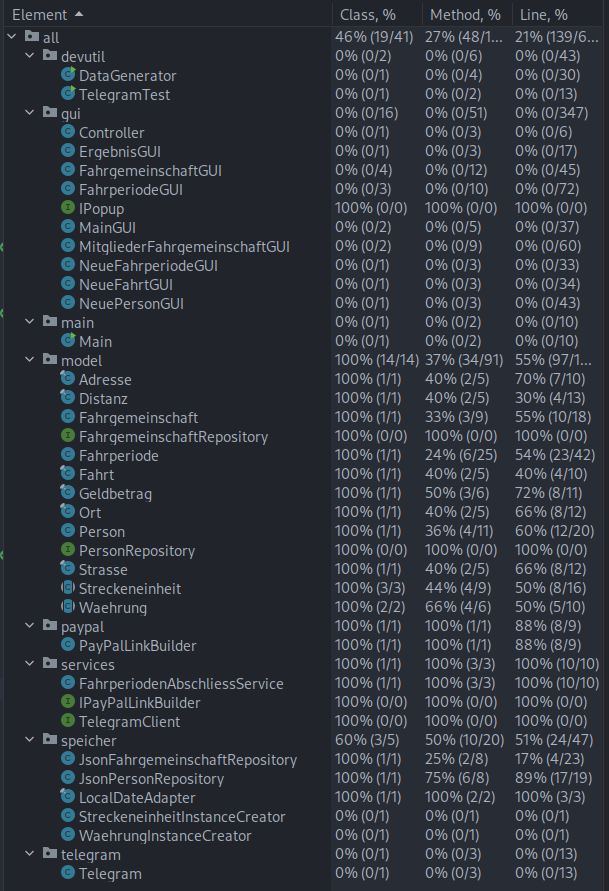
\includegraphics[width=0.5\textwidth]{Bilder/Coverage.png}
    \caption{Coverage-Analyse des Projekts}
    \label{fig:coverage}
\end{figure}

\section{Einsatz von Mocks}
Mocks werden bei Unit-Tests eingesetzt, um Abhängigkeiten während eines Tests zu ersetzen.
So hängt beispielsweise das Ergebnis eines Tests nicht von einer externen Datenbank ab.
Weiterhin könnte so auch einer Kopplung, wie im letzten Absatz beschrieben, entgegengewirkt werden.

Im Programmentwurf wurden in mehreren Tests Mocks eingesetzt.
Besonders gut zu sehen ist dies in den \href{https://github.com/yschiebelhut/carpool-java/blob/6d938e78763ca42270aafb8f51de4104c88e558a/0-carpool-java-plugin-json/src/test/java/speicher/LocalDateAdapterTest.java}{Tests des \code{LocalDateAdapters}}.
Hier wird bei beiden Tests mittels Mocks vermieden, dass ein echter JsonReader/-Writer erstellt werden muss, der wiederum einen Ein-/Ausgabestream voraussetzt -- beispielsweise aus einer Datei.

% ---- Literaturverzeichnis
\cleardoublepage
\renewcommand*{\chapterpagestyle}{plain}
\pagestyle{plain}
\pagenumbering{Roman}                   % Römische Seitenzahlen
\setcounter{page}{\numexpr\value{savepage}+1}
\printbibliography[title=Literaturverzeichnis]

% ---- Anhang
\appendix
%\clearpage
%\pagenumbering{Roman}  % römische Seitenzahlen für Anhang

\newpage
\end{document}
